\tikzset{every picture/.style={line width=0.75pt}} %set default line width to 0.75pt        

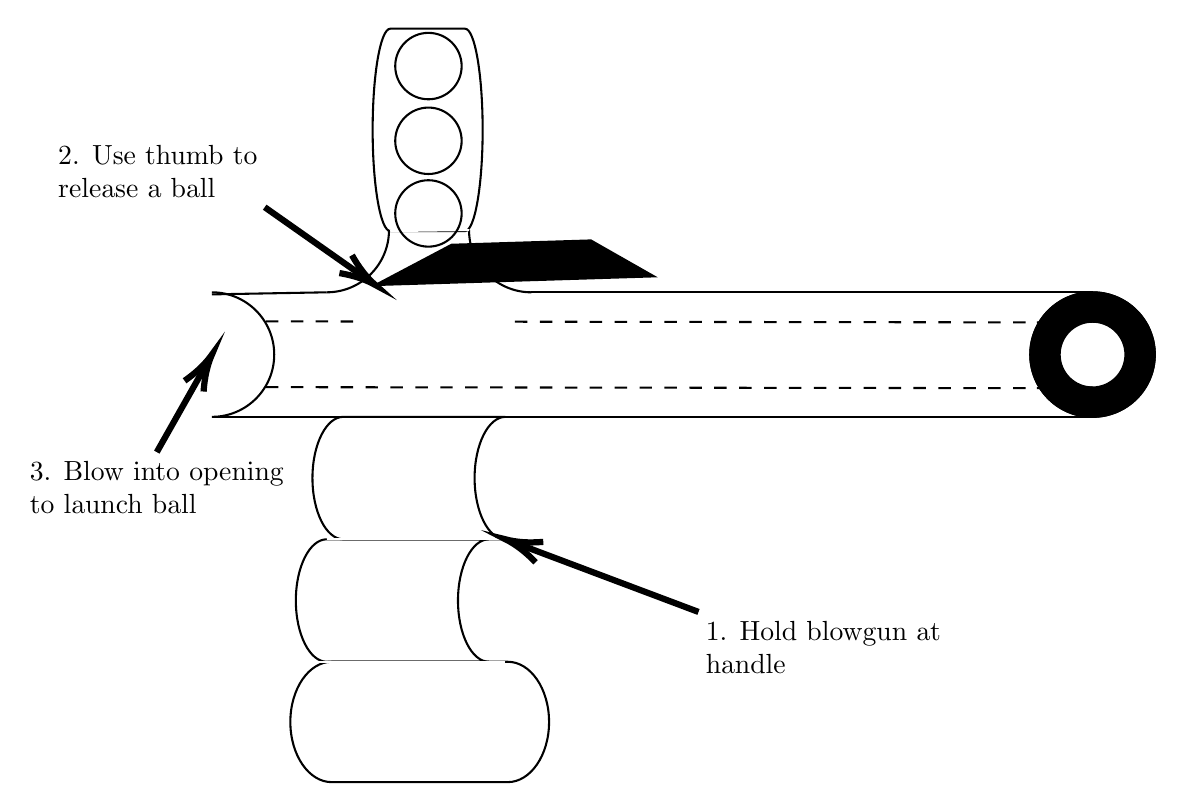
\begin{tikzpicture}[x=0.75pt,y=0.75pt,yscale=-1,xscale=1]
%uncomment if require: \path (0,375); %set diagram left start at 0, and has height of 375

%Flowchart: Stored Data [id:dp7020854973393003] 
\draw   (166.88,189) -- (245,189) .. controls (236.78,189) and (230.12,202.21) .. (230.12,218.5) .. controls (230.12,234.79) and (236.78,248) .. (245,248) -- (166.88,248) .. controls (158.66,248) and (152,234.79) .. (152,218.5) .. controls (152,202.21) and (158.66,189) .. (166.88,189) -- cycle ;
%Flowchart: Stored Data [id:dp17745579227095631] 
\draw   (158.88,248) -- (237,248) .. controls (228.78,248) and (222.12,261.21) .. (222.12,277.5) .. controls (222.12,293.79) and (228.78,307) .. (237,307) -- (158.88,307) .. controls (150.66,307) and (144,293.79) .. (144,277.5) .. controls (144,261.21) and (150.66,248) .. (158.88,248) -- cycle ;
%Flowchart: Terminator [id:dp12987464792265335] 
\draw   (161.29,307) -- (246.06,307) .. controls (257.07,307) and (266,319.98) .. (266,336) .. controls (266,352.02) and (257.07,365) .. (246.06,365) -- (161.29,365) .. controls (150.28,365) and (141.35,352.02) .. (141.35,336) .. controls (141.35,319.98) and (150.28,307) .. (161.29,307) -- cycle ;
%Shape: Boxed Line [id:dp02347467253997526] 
\draw    (386.42,189) -- (245,189) ;
%Shape: Boxed Line [id:dp07914747281461065] 
\draw    (527.84,189) -- (386.42,189) ;
%Shape: Arc [id:dp5416882594805525] 
\draw  [draw opacity=0] (527.84,189) .. controls (527.84,189) and (527.84,189) .. (527.84,189) .. controls (511.27,189) and (497.84,175.57) .. (497.84,159) .. controls (497.84,142.43) and (511.27,129) .. (527.84,129) .. controls (527.84,129) and (527.84,129) .. (527.84,129) -- (527.84,159) -- cycle ; \draw   (527.84,189) .. controls (527.84,189) and (527.84,189) .. (527.84,189) .. controls (511.27,189) and (497.84,175.57) .. (497.84,159) .. controls (497.84,142.43) and (511.27,129) .. (527.84,129) .. controls (527.84,129) and (527.84,129) .. (527.84,129) ;  
%Shape: Arc [id:dp5474126979604366] 
\draw  [draw opacity=0] (527.84,129) .. controls (527.84,129) and (527.84,129) .. (527.84,129) .. controls (544.41,129) and (557.84,142.43) .. (557.84,159) .. controls (557.84,175.57) and (544.41,189) .. (527.84,189) .. controls (527.84,189) and (527.84,189) .. (527.84,189) -- (527.84,159) -- cycle ; \draw   (527.84,129) .. controls (527.84,129) and (527.84,129) .. (527.84,129) .. controls (544.41,129) and (557.84,142.43) .. (557.84,159) .. controls (557.84,175.57) and (544.41,189) .. (527.84,189) .. controls (527.84,189) and (527.84,189) .. (527.84,189) ;  
%Shape: Boxed Line [id:dp7312749797342681] 
\draw    (527.84,129) -- (386.42,129) ;
%Shape: Boxed Line [id:dp6106897593312044] 
\draw    (386.42,129) -- (257.44,129) ;
%Shape: Arc [id:dp4419482433997406] 
\draw  [draw opacity=0] (257.44,129) .. controls (257.44,129) and (257.44,129) .. (257.44,129) .. controls (240.87,129) and (227.44,115.57) .. (227.44,99) -- (257.44,99) -- cycle ; \draw   (257.44,129) .. controls (257.44,129) and (257.44,129) .. (257.44,129) .. controls (240.87,129) and (227.44,115.57) .. (227.44,99) ;  
%Shape: Arc [id:dp9757784820393378] 
\draw  [draw opacity=0] (158.88,129) .. controls (175.45,129) and (188.88,115.57) .. (188.88,99) -- (158.88,99) -- cycle ; \draw   (158.88,129) .. controls (175.45,129) and (188.88,115.57) .. (188.88,99) ;  
%Shape: Diagonal Stripe [id:dp8622279132894688] 
\draw  [fill={rgb, 255:red, 0; green, 0; blue, 0 }  ,fill opacity=1 ] (286.14,104.01) -- (316.56,121.32) -- (182.32,125.49) -- (219.02,106.1) -- cycle ;
%Shape: Boxed Line [id:dp8393902716199675] 
\draw    (158.88,129) -- (103.58,130) ;
%Shape: Arc [id:dp8477854245084788] 
\draw  [draw opacity=0] (103.58,129) .. controls (120.15,129) and (133.58,142.43) .. (133.58,159) .. controls (133.58,175.57) and (120.15,189) .. (103.58,189) -- (103.58,159) -- cycle ; \draw   (103.58,129) .. controls (120.15,129) and (133.58,142.43) .. (133.58,159) .. controls (133.58,175.57) and (120.15,189) .. (103.58,189) ;  
%Shape: Boxed Line [id:dp3622748694370084] 
\draw    (245,189) -- (103.58,189) ;
%Straight Lines [id:da7926240509197231] 
\draw [color={rgb, 255:red, 255; green, 255; blue, 255 }  ,draw opacity=1 ][fill={rgb, 255:red, 255; green, 255; blue, 255 }  ,fill opacity=1 ]   (158.88,248) -- (245,248) ;
%Straight Lines [id:da2916687030607792] 
\draw [color={rgb, 255:red, 255; green, 255; blue, 255 }  ,draw opacity=1 ][fill={rgb, 255:red, 255; green, 255; blue, 255 }  ,fill opacity=1 ]   (158.88,248) -- (245,248) ;
%Straight Lines [id:da13038003848282242] 
\draw [color={rgb, 255:red, 255; green, 255; blue, 255 }  ,draw opacity=1 ][fill={rgb, 255:red, 255; green, 255; blue, 255 }  ,fill opacity=1 ]   (150.88,307) -- (237,307) ;
%Straight Lines [id:da7000012227824575] 
\draw [color={rgb, 255:red, 255; green, 255; blue, 255 }  ,draw opacity=1 ][fill={rgb, 255:red, 255; green, 255; blue, 255 }  ,fill opacity=1 ]   (158.88,307) -- (245,307) ;
%Flowchart: Terminator [id:dp8667157151263947] 
\draw   (189.48,2) -- (225.52,2) .. controls (230.2,2) and (234,23.83) .. (234,50.75) .. controls (234,77.67) and (230.2,99.5) .. (225.52,99.5) -- (189.48,99.5) .. controls (184.8,99.5) and (181,77.67) .. (181,50.75) .. controls (181,23.83) and (184.8,2) .. (189.48,2) -- cycle ;
%Straight Lines [id:da7095055647762649] 
\draw [color={rgb, 255:red, 255; green, 255; blue, 255 }  ,draw opacity=1 ][fill={rgb, 255:red, 255; green, 255; blue, 255 }  ,fill opacity=1 ]   (189.48,99.5) -- (227.44,99) ;
%Shape: Circle [id:dp006657138719728506] 
\draw   (191.88,20) .. controls (191.88,11.16) and (199.04,4) .. (207.88,4) .. controls (216.72,4) and (223.88,11.16) .. (223.88,20) .. controls (223.88,28.84) and (216.72,36) .. (207.88,36) .. controls (199.04,36) and (191.88,28.84) .. (191.88,20) -- cycle ;
%Shape: Circle [id:dp6645484876518424] 
\draw   (191.88,56) .. controls (191.88,47.16) and (199.04,40) .. (207.88,40) .. controls (216.72,40) and (223.88,47.16) .. (223.88,56) .. controls (223.88,64.84) and (216.72,72) .. (207.88,72) .. controls (199.04,72) and (191.88,64.84) .. (191.88,56) -- cycle ;
%Shape: Circle [id:dp2974845468289886] 
\draw   (191.88,91) .. controls (191.88,82.16) and (199.04,75) .. (207.88,75) .. controls (216.72,75) and (223.88,82.16) .. (223.88,91) .. controls (223.88,99.84) and (216.72,107) .. (207.88,107) .. controls (199.04,107) and (191.88,99.84) .. (191.88,91) -- cycle ;
%Straight Lines [id:da44337627056843143] 
\draw  [dash pattern={on 4.5pt off 4.5pt}]  (129.58,143) -- (501,143.5) ;
%Shape: Donut [id:dp5639385250613416] 
\draw  [fill={rgb, 255:red, 0; green, 0; blue, 0 }  ,fill opacity=1 ,even odd rule] (512,159) .. controls (512,150.25) and (519.09,143.16) .. (527.84,143.16) .. controls (536.59,143.16) and (543.69,150.25) .. (543.69,159) .. controls (543.69,167.75) and (536.59,174.84) .. (527.84,174.84) .. controls (519.09,174.84) and (512,167.75) .. (512,159)(497.84,159) .. controls (497.84,142.43) and (511.27,129) .. (527.84,129) .. controls (544.41,129) and (557.84,142.43) .. (557.84,159) .. controls (557.84,175.57) and (544.41,189) .. (527.84,189) .. controls (511.27,189) and (497.84,175.57) .. (497.84,159) ;
%Shape: Boxed Line [id:dp41615350387263916] 
\draw    (527.84,143.16) -- (501,143.5) ;
%Shape: Rectangle [id:dp7644990864790011] 
\draw  [color={rgb, 255:red, 255; green, 255; blue, 255 }  ,draw opacity=1 ][fill={rgb, 255:red, 255; green, 255; blue, 255 }  ,fill opacity=1 ] (175,129.5) -- (245,129.5) -- (245,169.5) -- (175,169.5) -- cycle ;
%Straight Lines [id:da8405108949064521] 
\draw  [dash pattern={on 4.5pt off 4.5pt}]  (129.58,174.69) -- (501,175.19) ;
%Shape: Boxed Line [id:dp6819604809628732] 
\draw    (527.84,174.84) -- (501,175.19) ;
%Straight Lines [id:da9497322294650778] 
\draw [line width=2.25]    (338,283) -- (248.74,249.41) ;
\draw [shift={(245,248)}, rotate = 20.62] [color={rgb, 255:red, 0; green, 0; blue, 0 }  ][line width=2.25]    (17.49,-5.26) .. controls (11.12,-2.23) and (5.29,-0.48) .. (0,0) .. controls (5.29,0.48) and (11.12,2.23) .. (17.49,5.26)   ;
%Straight Lines [id:da68271392613904] 
\draw [line width=2.25]    (129,88) -- (179.05,123.19) ;
\draw [shift={(182.32,125.49)}, rotate = 215.12] [color={rgb, 255:red, 0; green, 0; blue, 0 }  ][line width=2.25]    (17.49,-5.26) .. controls (11.12,-2.23) and (5.29,-0.48) .. (0,0) .. controls (5.29,0.48) and (11.12,2.23) .. (17.49,5.26)   ;
%Straight Lines [id:da4765070016353259] 
\draw [line width=2.25]    (77,206) -- (101.61,162.48) ;
\draw [shift={(103.58,159)}, rotate = 119.49] [color={rgb, 255:red, 0; green, 0; blue, 0 }  ][line width=2.25]    (17.49,-5.26) .. controls (11.12,-2.23) and (5.29,-0.48) .. (0,0) .. controls (5.29,0.48) and (11.12,2.23) .. (17.49,5.26)   ;

% Text Node
\draw (340,286) node [anchor=north west][inner sep=0.75pt]   [align=left] {1. Hold blowgun at\\handle};
% Text Node
\draw (127,85) node [anchor=south east] [inner sep=0.75pt]   [align=left] {2. Use thumb to\\release a ball};
% Text Node
\draw (77,209) node [anchor=north] [inner sep=0.75pt]   [align=left] {3. Blow into opening \\to launch ball};


\end{tikzpicture}
